\newpage
\section{Data Sources and Models}

% \tiny \begin{verbatim}
%   Misun, Paul, Tzanio, Dillon  (pay attn to APPENDIX 2)
%
%   Describe which existing or new data sources will be used. Address your team’s access to the data.
%   If applicable, indicate which AI models or frameworks will be used in your proposed project.
%   Do not include a computing resources--to be done in Appendix 2.
%
%   Here, discuss: o  Experimental data for fuel pins \cite{KAERI,Todreas}
%                  o  Nek5000/RS and MFEM as trusted high-accuracy and efficient sources
%                  - Top-ranked in numerous benchmark cases (T-junction \cite{tjunc}, 5x5-pin spacer grid \cite{5pin}, etc.)
%                  - 1/32 the amount of computational resources as FV for the same accuracy for Re=50M
%                    boundary layer calculation (1/8 the number of grid points, 1/2 the number of timesteps,
%                    and 1/2 the time per step, per gridpoint on the same platform, OLCF Summit)
%
%  o  Collins data for the small wire-coil - both experimental and numerical results available
% \end{verbatim}
%
% \normalsize

%%%%%%%%%%%%%%%%%%%%%%%%%%%%%
\begin{wrapfigure}{rb}{0.30\textwidth}
\vspace{-2pt}
\centering
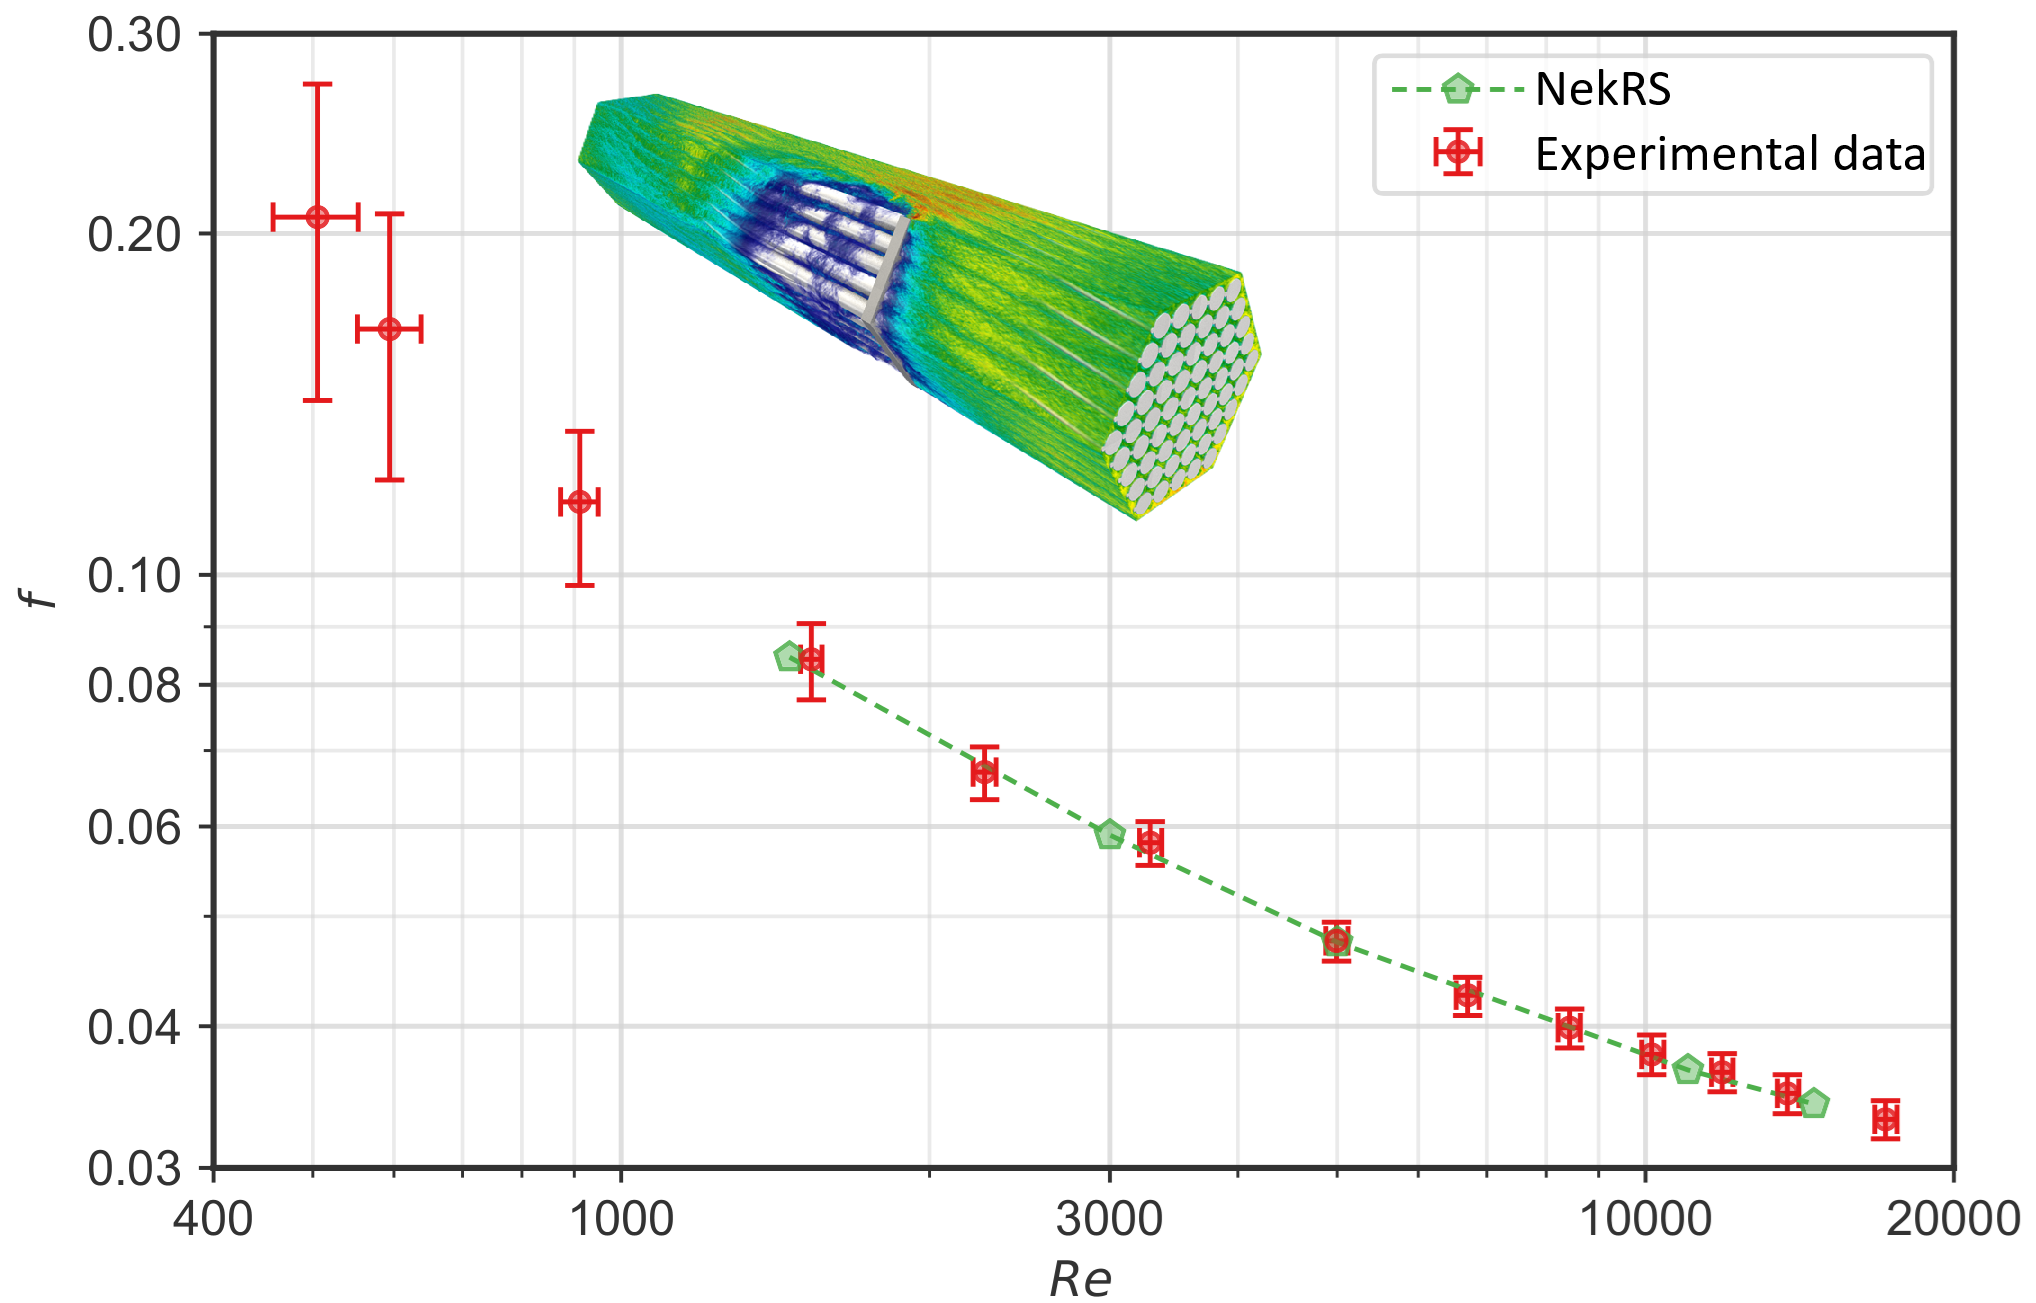
\includegraphics[width=0.30\textwidth]{../figs/dai_data.png}
%vspace{-2pt}
\caption{\label{fig:blocked}
Experimental-NekRS data comparison of friction factor vs. Reynolds number 
for a wire-wrapped bundle with blockage \cite{Dai2025WireWrapped61Pin}.
}
\end{wrapfigure}
%%%%%%%%%%%%%%%%%%%%%%%%%%%%%
The Argonne team has extensive experience in LES of turbulent flow in liquid
metal fast reactors, spanning configurations from isolated subassemblies
\cite{fischer08a,Dai2025WireWrapped61Pin,shaver37pin,shavernacie} to 
full-core reactor geometries~\cite{sc22,gb23}.  
The majority of these datasets are available for immediate use
They are well-documented in the nuclear design literature and provide validated
benchmarks for thermal–fluid performance prediction.  
  In particular, we have access to {\em experimentally validated}
datasets for a 61-pin assembly over a range of Reynolds numbers
\cite{Dai2025WireWrapped61Pin}, as well as datasets for a 19-pin assembly under
multiple flow and heating conditions~\cite{shavernacie}.  
  Similarly, the MFEM team possesses high-resolution simulation datasets
from model ICF studies spanning wide range of operating
regimes, geometries and spatial resolutions.  
{\bf Both Nek5000/RS and MFEM have infrastructure to automatically 
produce additional data on HPC platforms, including Frontier and Aurora, 
as part of ongoing studies.}
These efforts include simulations of
7-pin reflector assemblies and 37-pin configurations similar to those
studied by Shaver~\cite{shaver37pin}.  Recent highly-detailed
experimental datasets for wire-wrapped bundles are available in~\cite{kaeri37pin},
and will be incorporated into model training and validation.  
%%   The generation of wire-wrapped fuel bundle geometries has been fully automated,
%% enabling rapid sampling of new points in the wire-wrap geometry space and
%% systematic expansion of the training dataset.

\begin{wrapfigure}{rb}{0.30\textwidth}
\vspace{-2pt}
\centering
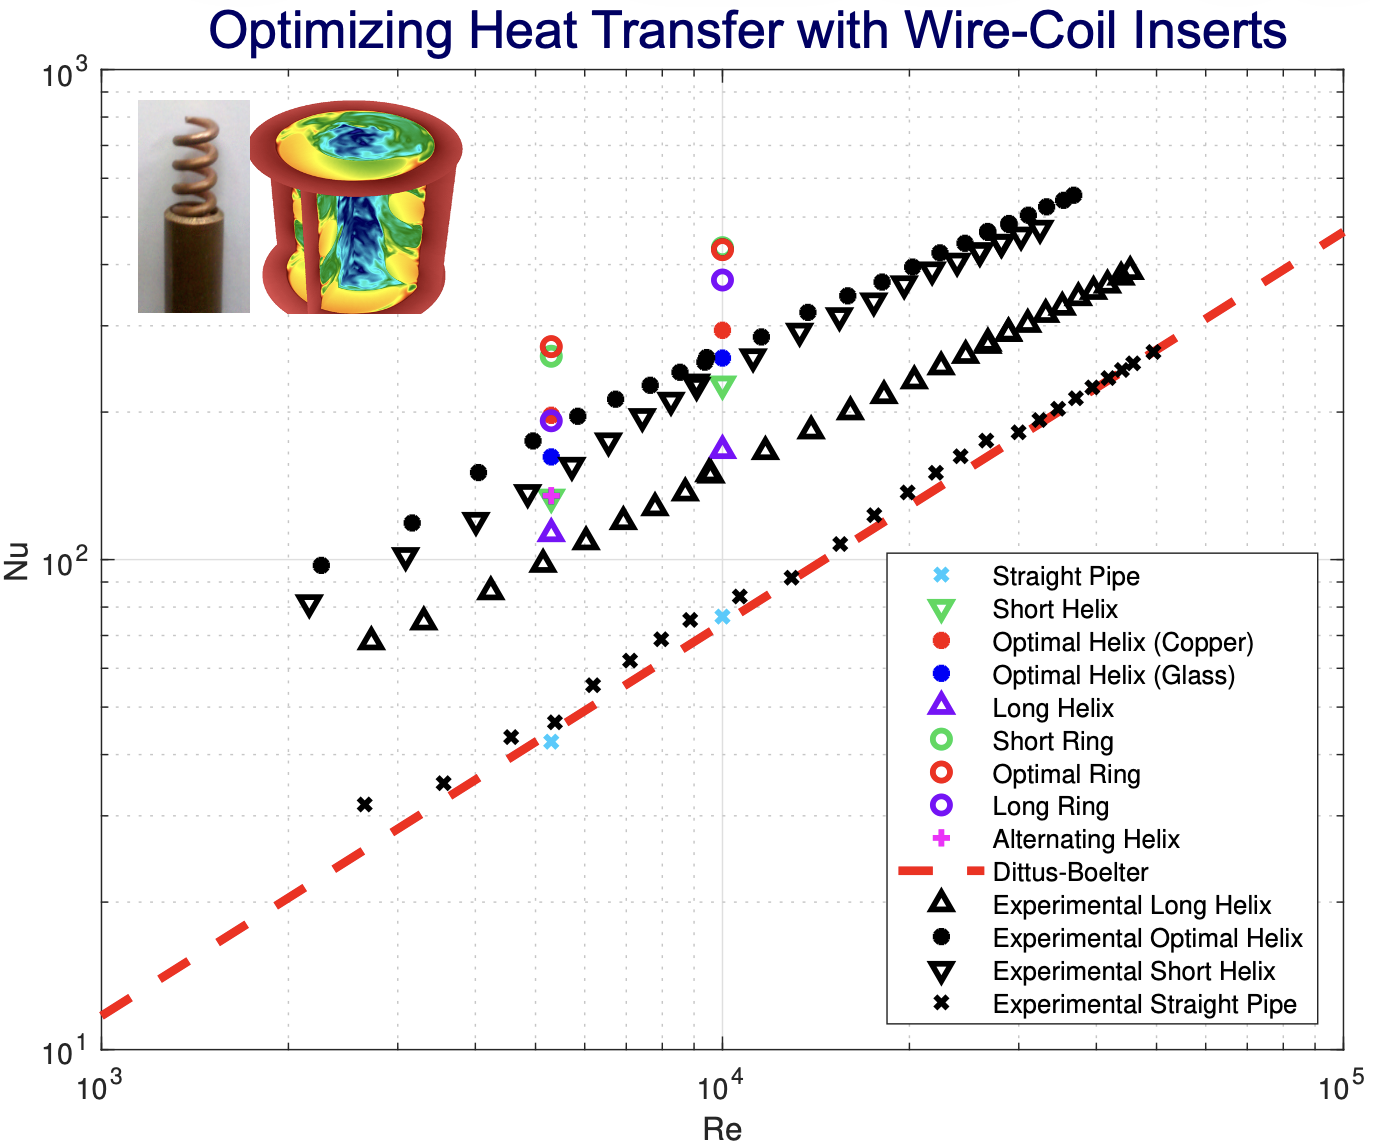
\includegraphics[width=0.29\textwidth]{../figs/collins_02_nek_nu3_new.png}
\caption{\label{fig:collins}
Experimental-Nek5000 /RS data comparison of Nusselt 
vs. Reynolds number for wire-coil insert geometries \cite{kaneko22}.
}
\vspace{-7pt}

\end{wrapfigure}
%%%%%%%%%%%%%%%%%%%%%%%%%%%%
A similar data-generation framework exists for wire-coil insert geometries, 
which provide a low-cost model for workflow testing and method development.  
% The data situation is similar for the wire-coil insert geometry, which is a
% low-cost case to be used for test/development of the overall workflow.
Extensive high-quality experimental datasets are available in \cite{collins22}
and have been corroborated through Nek5000/RS simulations by Kaneko \cite{kaneko22}, 
including studies of related configurations such as arrays of ring inserts.
%
% These cases are computationally inexpensive and can typically be executed on
% one or two GPUs within approximately one hour to generate requisite QOIs, such
% as the Nusselt number (Nu), a nondimensional heat-transfer coefficient.
% Importantly, the Nusselt number in these configurations
% exhibits strong sensitivity to geometric variation, with increases of up to
% fourfold observed in both experiments and simulations for optimized geometries.
% This strong geometry–performance coupling provides an ideal testbed for
% evaluating automated AI-driven optimization workflows and demonstrating
% measurable performance gains.
%
These cases are relatively small and can be run on one or two GPUs for one hour
to generate requisite QOIs (e.g., Nusselt number, Nu, which is the
nondimensional heat-transfer coefficient).  It is also a case where the QOI is
sensitive to geometry, with up to a 4$\times$ increase in Nu observed in
experiments and simulations for the best configurations, implying that there is
a significant performance benefit that should be identifiable by the automated
AI optimization framework.



%%%%%%%%%%%%%
%It is also a case where the QOI is
%sensitive to geometry, with up to a 4$\times$ increase in Nu observed in
%experiments and simulations for the best configurations, implying that there 
%is a significant performance benefit that should be identifiable
%by the automated AI optimization framework.
%%%%%%%%%%%%%%%

